\documentclass[]{beamer}

%%% BEAMER SETUP %%%

\usetheme{Rochester}
\usecolortheme{seahorse}

\beamertemplatenavigationsymbolsempty

\title[Preprocessing techniques for UATR]{Experiments in preprocessing techniques for underwater acoustic target recognition}
\author[Antriksh Dhand]{\texorpdfstring{\textbf{Antriksh Dhand}\\{\small Supervised by Dr.~Dong Yuan}}{\textbf{Antriksh Dhand}}}
\date{February 28th, 2025}

\institute[USYD]
{
    School of Electrical and Computer Engineering\\
    The University of Sydney
}

\AtBeginSection[]
{
    \begin{frame}
        \frametitle{Table of Contents}
        \tableofcontents[currentsection]
    \end{frame}
}

\AtBeginSubsection[] {
    \begin{frame}
        \frametitle{Table of Contents} %
        \tableofcontents[currentsection, currentsubsection]  
    \end{frame}
}

%%% PACKAGES %%%

\usepackage{hyperref}
\usepackage[dvipsnames]{xcolor}
\usepackage{booktabs}
\usepackage{multirow}
\usepackage{graphicx}
\usepackage{tikz}
\usetikzlibrary{shapes, arrows.meta, positioning, calc}
\usepackage{caption}
\usepackage{subcaption}

\setbeamerfont{footnote}{size=\scriptsize}

%%%%%%%%%%%%%%%%%%%%%%%%%

\begin{document}

\begin{frame}
    \titlepage
\end{frame}

%===============================================================================
% INTRODUCTION 
%===============================================================================

\section{Introduction}

\begin{frame}{Background}
    \begin{exampleblock}{Underwater Acoustic Target Recognition (UATR)}
        UATR is the analysis of a sonar signal with the aim of determining its source.
    \end{exampleblock}
    \vspace{0.5cm}
    \begin{columns}
        \begin{column}{0.55\textwidth}
            Current approaches are manual, with acoustic data being analysed by human sonar operators.

            \vspace{0.25cm}
            
            This thesis focuses on the automation of UATR using machine learning techniques, particularly deep learning methods.
            
        \end{column}
        \begin{column}{0.45\textwidth}
            \begin{figure}
                \centering
                \includegraphics[trim={2cm 0 2cm 0},clip,width=\textwidth]{img/sonar_operator.jpeg}
            \end{figure}
        \end{column}
    \end{columns}
\end{frame}

% \begin{frame}{Background}
%     This thesis focuses on the automation of UATR using machine learning techniques, particularly deep learning methods.
%     \vspace{0.5em}
%     \begin{figure}
%         \centering
%         \includegraphics[width=0.7\textwidth]{img/uatr_flowchart.png}
%         % Everything in the second half of the image is currently done by humans
%     \end{figure}
%     %But there are many challenges in applying ML in this domain.
% \end{frame}

% \begin{frame}{Challenges in UATR}
%     Recall the recipe for progress in computer vision in the 2010s:
%     \begin{enumerate}
%         \item Big data
%         \item Big compute
%         \item Big access
%     \end{enumerate}
%     % Big data: There are only 3 publically available datasets.
%     % Big compute: Are we sure CNNs are the best way to handle audio/sonar data? This whole thing is essentially just some crazy form of transfer learning.
%     % Big access: In the 2010s, literally anyone could contribute to making models better because anyone can identify objects in an image. You cannot do the same with sonar recordings.

%     \begin{columns}
%         \begin{column}{0.4\textwidth}
%             \small
%             All three factors are limited in the underwater acoustic domain, but the most critical challenge is the scarcity of large, high-quality, labelled datasets.
%         \end{column}
%         \begin{column}{0.6\textwidth}
%             \begin{table}[]
%                 \scriptsize
%                 \captionsetup{font=scriptsize}
%                 \setlength{\belowcaptionskip}{0pt}
%                 \caption{Volume of common ML audio datasets}    
%                 \resizebox{\linewidth}{!}{  % Resize table to fit within the column
%                 \begin{tabular}{@{}llll@{}}
%                 \toprule
%                 \textbf{Domain} & \textbf{Dataset} & \textbf{Recordings} & \textbf{Hours} \\ \midrule
%                 \multirow{2}{*}{Underwater} & ShipsEar & 90 & 3 \\
%                  & Deepship & 613 & 47 \\ \midrule
%                 \multirow{3}{*}{In-air} & FSD50K & 51,197 & 108 \\
%                  & AudioSet & 1,789,621 & 4,971 \\
%                  & Common Voice & 13,000,000 & 18,000 \\ \bottomrule
%                 \end{tabular}
%                 }
%             \end{table}
%         \end{column}
%     \end{columns}
% \end{frame}

\begin{frame}{Challenges in UATR}
    The most critical challenge facing UATR research is the scarcity of large, high-quality, labelled datasets. 

    \vspace{0.5cm}
    
    \begin{table}[]
        \scriptsize
        \captionsetup{font=scriptsize}
        \setlength{\belowcaptionskip}{0pt}
        \caption{Volume of common ML audio datasets}    
        \begin{tabular}{@{}llll@{}}
        \toprule
        \textbf{Domain} & \textbf{Dataset} & \textbf{Recordings} & \textbf{Hours} \\ \midrule
        \multirow{2}{*}{Underwater} & ShipsEar & 90 & 3 \\
         & Deepship & 613 & 47 \\ \midrule
        \multirow{3}{*}{In-air} & FSD50K & 51,197 & 108 \\
         & AudioSet & 1,789,621 & 4,971 \\
         & Common Voice & 13,000,000 & 18,000 \\ \bottomrule
        \end{tabular}
    \end{table}
\end{frame}

\begin{frame}{Challenges in UATR}
   \framesubtitle{Lack of high-quality, labelled datasets}

   \textbf{Why is gathering labelled underwater acoustic data so difficult?}
   \begin{itemize}
        \item Resource-intensive and costly: requires time, equipment, maritime logistical coordination, and legal clearance.
        \item Curation and annotation are highly specialised.
        \item Many recordings are classified, especially military-related.
   \end{itemize}

   \vspace{0.3cm}
   \textbf{Why are underwater recordings prone to being low-quality?}
    \begin{itemize}
        \item Signal attenuation (refraction, absorption, scattering, geometrical spreading losses, etc.)
        \item Multipath propagation leading to delays and signal distortion
        \item Ambient noise interference interferes with true signal
    \end{itemize}
\end{frame}

\begin{frame}{Motivation}

    \begin{center}
    \textbf{\Large Preprocessing could help UATR work with limited, noisy data.}
    \end{center}

    \vspace{0.5cm}
    
    \begin{figure}
        \centering
        \includegraphics[width=0.8\linewidth]{img/methodology_flowchart_3.png}
    \end{figure}
\end{frame}

\begin{frame}{Aim}

    This thesis investigates the impact of three preprocessing techniques on UATR classification accuracy using the DeepShip dataset.

    \vspace{0.5cm}

    \begin{columns}
        \begin{column}{0.33\textwidth}
            \begin{block}{Normalisation}
                Adjusts signal amplitudes for consistency.
            \end{block}
        \end{column}
        \begin{column}{0.33\textwidth}
            \begin{block}{Detrending}
                Removes long-term trends to highlight periodic features.
            \end{block}
        \end{column}
        \begin{column}{0.33\textwidth}
            \begin{block}{Denoising}
                Reduces ambient noise for clearer signal interpretation.
            \end{block}
        \end{column}
    \end{columns}

\end{frame}

%===============================================================================
% Methodology
%===============================================================================

\section{Methodology}

\begin{frame}{Building a benchmark classifier}
    To isolate the effect of each preprocessing technique on signal quality, we first establish a baseline measure of performance with a fixed classification model.
    \vspace{0.25cm}
    \begin{figure}
        \centering
        \includegraphics[width=\linewidth]{img/methodology_flowchart_2.png}
    \end{figure}
\end{frame}

\begin{frame}{Input data}

    All experiments used DeepShip, the authoritative benchmark dataset for UATR. 

    \vspace{0.25cm}
    
    \begin{columns}
        \begin{column}{0.35\textwidth}
            \begin{itemize}
                \item Recordings were segmented into 53,503 3-second clips to boost training samples and manage computational complexity.
                \item Segments were divided into 10 folds.
            \end{itemize}
        \end{column}

        \begin{column}{0.65\textwidth}
            \centering
            \includegraphics[width=\linewidth]{img/10_class_counts_facet.pdf}
        \end{column}
    \end{columns}

    % \begin{itemize}
    %     \item All clips from a recording were placed in the same fold.
    %     \item Efforts were made to **balance vessel samples** across folds.
    % \end{itemize}
\end{frame}

% \begin{frame}{Input data}
%     All experiments used DeepShip, the authoritative benchmark dataset for UATR. 
%     \begin{itemize}
%         \item The recordings were segmented into 53,503 3-second segments to boost training samples and manage computational complexity.
%         \item These segments were divided into 10 folds.
%         \begin{itemize}
%             \item All clips from a given recording were placed in the same fold.
%             \item An effort was made to distribute an equal number of samples from each vessel into each fold.
%         \end{itemize}
%     \end{itemize}
% \end{frame}

% \begin{frame}[plain]{}
%     % Due to inherent imbalance in recording durations, it was not perfect
%     % e.g. Tug shows the greatest variation between folds, but that is because it has by far the least number of ships, least number of recordings, but the recordings are very long.
%     \begin{figure}
%         \captionsetup{font=scriptsize}
%         \centering
%         \includegraphics[width=\textwidth]{img/10_class_counts_facet.pdf}
%         \vspace{-9pt}
%         \caption{Count of samples in each class by fold}
%     \end{figure}
% \end{frame}

\begin{frame}{Input features}
    \small
    \begin{exampleblock}{Power spectrogram}
    A transformed version of the conventional spectrogram $S$, calculated as $10 \cdot \log_{10}(|S|^2 + \epsilon)$, designed to enhance interpretability and better align with human auditory perception.
    \end{exampleblock}

    \begin{figure}
        \centering
        \includegraphics[width=0.5\linewidth]{img/Tug.png}
    \end{figure}

\end{frame}

\begin{frame}{Input features}
    \framesubtitle{Processing pipeline}
    \begin{enumerate}
        \item Downsample \texttt{.wav} file to 5 kHz 
        \item Perform 0-1 amplitude normalisation
        \item Generate spectrogram 
        {\scriptsize
            \begin{table}[htbp]
                \centering
                \begin{tabular}{@{}ll@{}} \toprule 
                \textbf{Parameter} & \textbf{Value} \\ \midrule 
                Sampling frequency (\texttt{fs}) & 5 kHz \\ 
                Window length (\texttt{window}) & 40 ms = 200 segments, rounded to 256 \\ 
                Overlap (\texttt{noverlap}) & 75\% of window length \\ 
                Fast Fourier transform length (\texttt{nfft}) & 1024 points \\ 
                Output dimensions & $195 \times 231$ (frequency bins $\times$ time bins) \\ \bottomrule
                \end{tabular}
            \end{table}
        }
        \item Amplitude cutoff below $-30$ dB
        \item Frequency cutoff below $50$ Hz and $1000$ Hz
        \item Resize to $192 \times 192$
        \item Export as \texttt{.mat} files
    \end{enumerate}
\end{frame}

\begin{frame}{The CNN-LSTM classifier}
    \small
    A hybrid \textbf{convolutional neural network--long short-term memory (CNN-LSTM)} classifier was chosen to leverage the strengths of both CNNs for spatial feature extraction and LSTM networks for sequential data processing.

    % Mention hyperparameter tuning with KerasTuner
    
    \begin{figure}
        \centering
        \includegraphics[width=0.9\textwidth]{img/architecture_diagram.pdf}
    \end{figure}
    \begin{center}
		Ultimately, the baseline CNN-LSTM model achieved an overall accuracy of \textbf{63.41\%} after 5 epochs.
	\end{center}
\end{frame}

% \begin{frame}{The CNN-LSTM classifier}
    
%     Hyperparameter tuning was performed using \texttt{KerasTuner} to find the most promising model architecture and training configuration.
%     \begin{table}
%         \scriptsize
%         \captionsetup{font=scriptsize}
%         % \setlength{\belowcaptionskip}{0pt}
        
%         \centering
%         \caption{Final training parameters for benchmark CNN-LSTM model.}
%         \begin{tabular}{ll}
%         \toprule
%         \textbf{Parameter} & \textbf{Final value} \\ \midrule
%         GPU batch size & 16 \\
%         Optimiser & Adam \\
%         Loss function & Categorical cross-entropy \\
%         Learning rate & $1 \times 10^{-5}$ \\
%         Validation approach & Leave-two-out 10-fold cross validation \\
%         Evaluation metrics & Accuracy, F1-score \\ \bottomrule
%         \end{tabular}
%     \end{table}
    
%     \begin{center}
% 		Ultimately, the baseline CNN-LSTM model achieved an overall accuracy of \textbf{63.41\%} after 5 epochs.
% 	\end{center}
% \end{frame}

% \begin{frame}[plain]{The CNN-LSTM classifier}
%     \centering
%     \includegraphics[trim={3cm 0 3cm 0.8cm}, clip, width=0.9\linewidth]{img/cnn_lstm_by_epoch.pdf}
%     \includegraphics[trim={3cm 0 3cm 0.8cm}, clip, width=0.9\linewidth]{img/cnn_lstm_by_fold.pdf}
% \end{frame}


%===============================================================================
% Experiments 
%===============================================================================

\section{Experiments and results}

%---------------------------- Normalisation -----------------------------------
\subsection{Normalisation}

\begin{frame}{Overview}
    \begin{block}{Hypothesis}
    Normalisation improves UATR performance by ensuring all inputs share similar statistical properties, helping maintain a uniform and stable gradient flow throughout the neural network.
    \end{block}
    \vspace{0.2cm}
    \input{cube_comparison}
    % Talk about implementation
\end{frame}

\begin{frame}[plain]{}
    \centering
    \includegraphics[width=\linewidth]{img/spectrogramComparison.pdf}
    
    \vspace{0.3cm}
    
    \includegraphics[clip,trim={0 0 0 0.6cm},width=\linewidth]{img/histogramComparison.pdf}
\end{frame}

\begin{frame}{Results}
    \textbf{There were minimal differences between each normalisation strategy.}
    
    \vspace{0.5cm}
    
    \begin{table}
    \scriptsize
    \captionsetup{font=scriptsize}
    \centering
    \caption{Accuracy comparison of normalisation strategies on the DeepShip dataset}
    \begin{tabular}{@{}lc@{}}
        \toprule
        \textbf{Normalisation strategy} & \textbf{Accuracy (\%)} \\
        \midrule
        Global normalisation            & 62.99 \\
        Channel-based normalisation     & 63.16 \\
        \textbf{Baseline} & \textbf{63.41} \\
        \bottomrule
    \end{tabular}
    \end{table}
\end{frame}

\begin{frame}{Discussion}
    \begin{alertblock}{Why didn't normalisation work as expected?}
        \begin{itemize}
            \item Power spectrogram may have already standardised the data, reducing the effects of additional normalisation.
            \item The controlled recording setup (fixed hydrophone) led to uniform feature scales, diminishing the effect of normalisation.
        \end{itemize}
    \end{alertblock}

    \begin{block}{Future work}
        \begin{itemize}
            \item Investigate alternative normalisation techniques (e.g. 0-1 normalisation, local normalisation).
            \item Explore datasets with greater variability (e.g. towed array recordings).
        \end{itemize}
    \end{block}
\end{frame}

%---------------------------- Detrending -------------------------------------
\subsection{Detrending}

\begin{frame}{Overview}
    \begin{block}{Hypothesis}
        Detrending improves UATR performance by suppressing broadband noise and highlighting transient features important for classification. %such as the period signals generated by ship machinery.
    \end{block}
    
    \small
    The $\ell_1$ detrending algorithm modifies the traditional Hodrick-Prescott filter by using an $\ell_1$ norm $(\| \cdot \|)$ for smoothness:
    \begin{equation*}
        \frac{1}{2} \sum_{t=1}^n (y_t - x_t)^2 + \lambda \sum_{t=2}^{n-1} \| x_{t-1} - 2x_t + x_{t+1} \|
    \end{equation*}
    \vspace{-7pt}
    \begin{itemize}
        \item $\lambda$ controls smoothing: higher values detrend more aggressively, lower values retain variability.
        \item By fine-tuning $\lambda$ we can strike a balance between removing the trend and preserving the narrowband features critical for classification.
    \end{itemize}
\end{frame}

\begin{frame}{Implementation}

    \begin{itemize}
        \item Built on the original MATLAB implementation of the $\ell_1$ detrending algorithm.
        \item Defined regularisation strength $\lambda$ as a fraction $\alpha$ of $\lambda_{\text{max}}$ (upper bound for detrending).
        \item Trained CNN-LSTM model on detrended spectrograms using $\alpha = 10^{-2}$, $10^{-1}$, $1$.
    \end{itemize}
\end{frame}

\begin{frame}[plain]{}
    \begin{figure}
        \captionsetup{font=scriptsize}
        \centering
        \includegraphics[width=\linewidth]{img/segment_l1_trend.pdf}
        \caption{Overlay of a time segment with its corresponding $\ell_1$ trend at various $\alpha$ values}
    \end{figure}
\end{frame}

% \begin{frame}[plain]{}
%     \begin{figure}
%         \captionsetup{font=scriptsize}
%         \centering
%         \includegraphics[width=\linewidth]{img/segment_detrended.pdf}
%         \caption{A time segment before and after detrending at various $\alpha$ values}
%     \end{figure}
% \end{frame}

% \begin{frame}[plain]{}
%     \begin{figure}
%         \captionsetup{font=scriptsize}
%         \centering
%         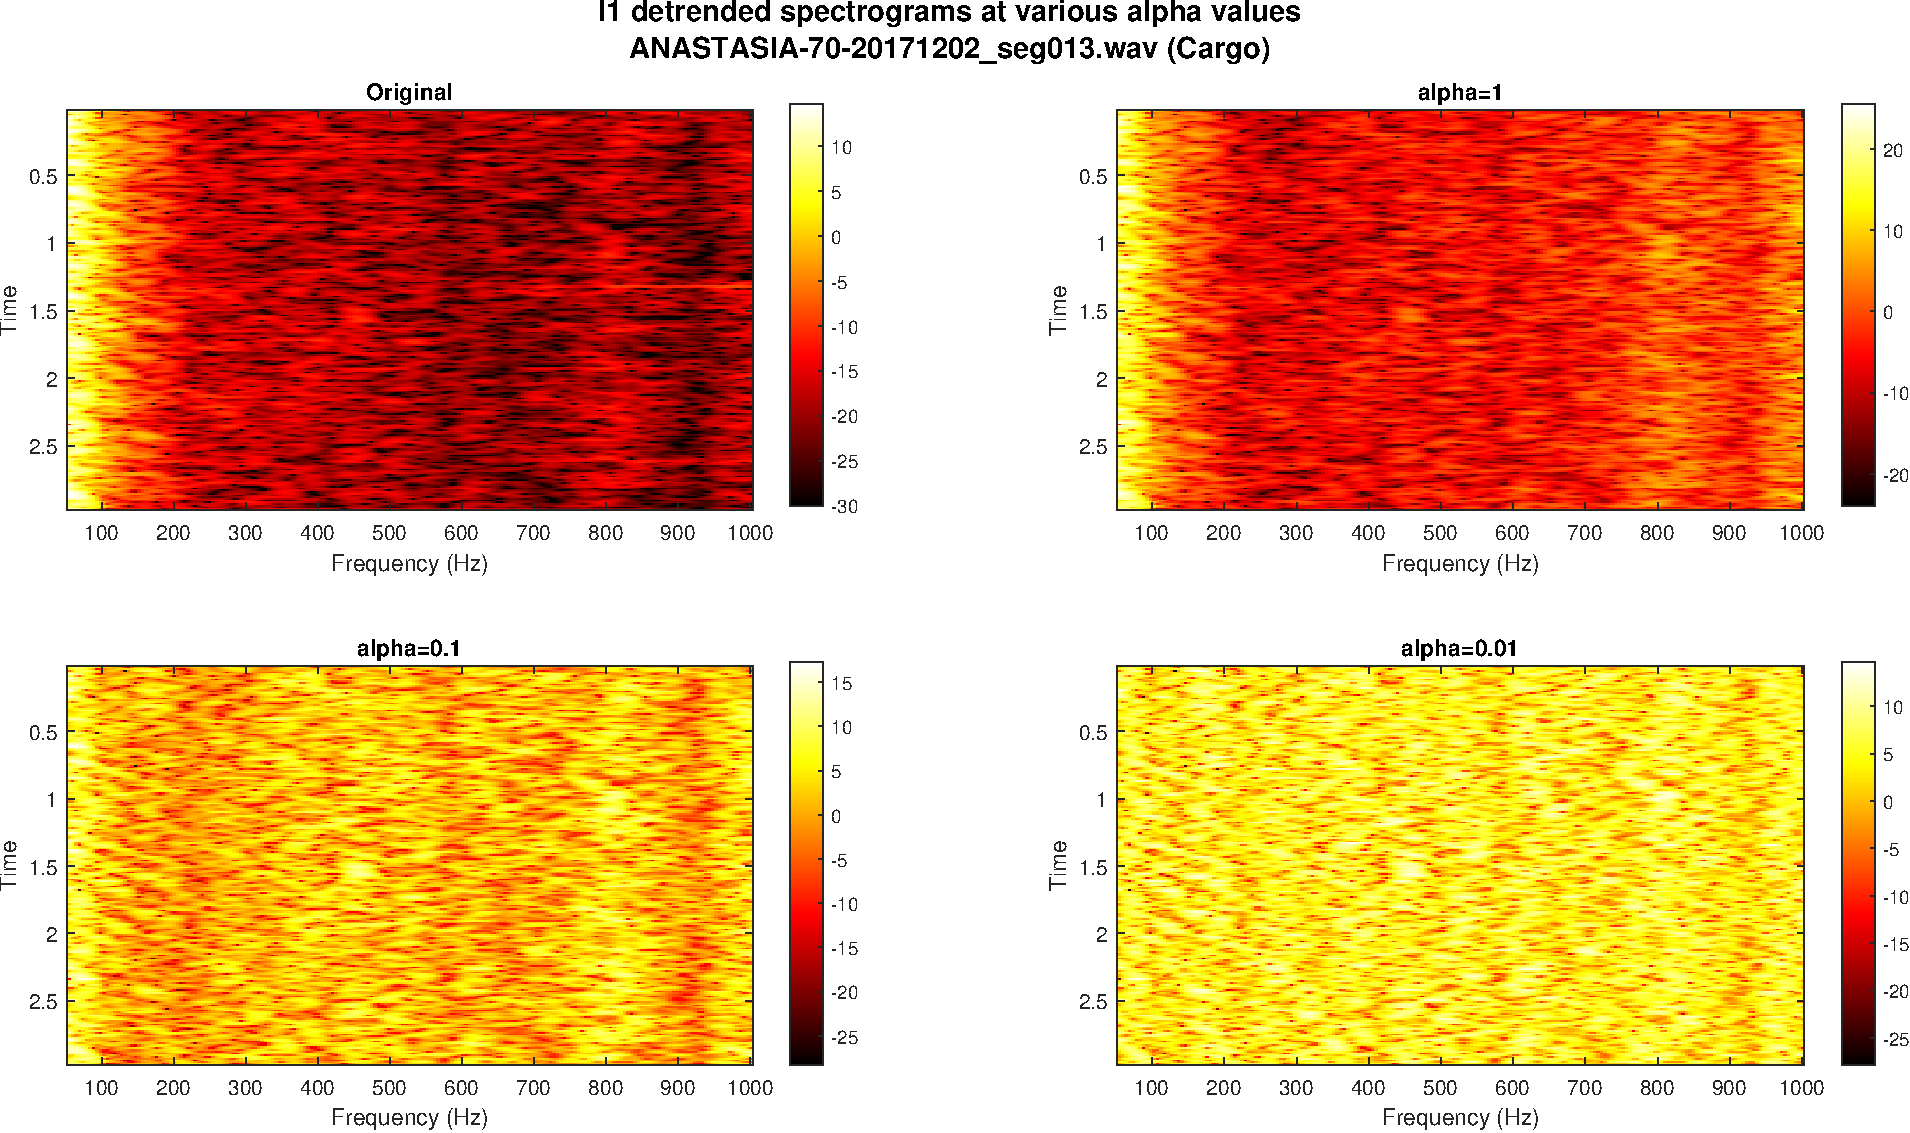
\includegraphics[width=\linewidth]{img/spec_comparison.pdf}
%         \caption{Comparison of original and detrended spectrograms at various $\alpha$ values}
%     \end{figure}
% \end{frame}

\begin{frame}{Results}

    \textbf{All three detrending configurations resulted in lower classification accuracy compared to the baseline.}

    \vspace{0.5cm}

    \begin{table}[htbp]
    \scriptsize
    \captionsetup{font=scriptsize}
    \centering
    \caption{Classification results using $\ell_1$ detrending algorithm at various $\alpha$}
    \begin{tabular}{@{}lc@{}}
        \toprule
        \textbf{Detrending parameter} & \textbf{Accuracy (\%)} \\ \midrule
        $\alpha = 10^{-2}$            & 48.22 \\
        $\alpha = 10^{-1}$            & 52.03 \\
        $\alpha = 1$                  & 55.63 \\
        \textbf{Baseline (no detrending)}  & \textbf{63.41} \\
        \bottomrule
    \end{tabular}
\end{table}
\end{frame}

\begin{frame}{Discussion}
    \small
    \begin{alertblock}{Why didn't detrending work as expected?}
        \begin{itemize}
            \item The short segment duration of 3s may have prevented accurate trend estimation.
            \item Detrending altered spatial and temporal characteristics, potentially hindering the CNN-LSTM model's learning.
            \item Low values of $\alpha$ may have been over-smoothing, while high values of $\alpha$ may have been under-suppressing. 
        \end{itemize}
    \end{alertblock}

    \begin{block}{Future work}
        \begin{itemize}
            \item Investigate detrending's impact with different model architectures.
            \item Experiment with longer audio segments to improve trend estimation.
            \item Compare $\ell_1$ detrending to alternative methods (e.g. wavelet-based detrending).
        \end{itemize}
    \end{block}
\end{frame}

%---------------------------- Denoising --------------------------------------
\subsection{Denoising}

\begin{frame}{Overview}
    \begin{columns}
        \begin{column}{0.42\textwidth}
            \small This experiment aims to uncover the efficacy of deep learning-based \textbf{image denoising techniques} for underwater acoustic spectrograms.
        \end{column} 
        \begin{column}{0.58\textwidth}
            \begin{figure}
                \centering
                \includegraphics[width=\linewidth]{img/denoising_family.png}
            \end{figure}
        \end{column} 
    \end{columns}
    
    % \textbf{Challenges:}
    % \begin{itemize}
    %     \item Lack of hydrophone array recordings
    %     \item Complex noise patterns and interactions
    %     \item Variability of the underwater acoustic environment
    % \end{itemize}
\end{frame}

% \begin{frame}{Overview}
%             \begin{block}{Hypothesis}
%             Denoising improves UATR performance by removing ambient noise which can mask or distort the original signal.
%             \end{block}
        
%     \alert{This part of my thesis aims to explore whether image-based denoising techniques were transferrable to spectrograms, treating them as an image.}
    
%     \begin{enumerate}
%         \item Mapping-based techniques: learn a function which directly maps a noisy input to a clean output.
%         \setbeamertemplate{enumerate items}[default]
%         \begin{enumerate}
%             \item Supervised methods%: rely on paired clean and noisy data for training.
%             \item Unsupervised methods%: leverage properties of the noise distributions to perform denoising.
%         \end{enumerate}
%         \setbeamertemplate{enumerate items}[square]
%         \item Masking-based techniques: generate binary masks to highlight specific features which are later used for classification.
%     \end{enumerate}
% \end{frame}

\begin{frame}{Experiment 1: Unsupervised denoising with Noise2Noise}
    
    %Unsupervised methods leverage properties of the noise distributions or the inherent structure of the signal itself to perform denoising.

    \begin{exampleblock}{Noise2Noise (N2N)}
        The Noise2Noise model can learn to denoise images using only pairs of independently corrupted noisy images provided that 
        \begin{itemize}
            \item the noise has a zero-mean distribution, and
            \item the noise in the input and target images are uncorrelated.
        \end{itemize}
    \end{exampleblock}
    
    \begin{alertblock}{Objectives}
        \begin{enumerate}
            \item To validate the N2N approach by recreating its performance on natural images.
            \item To investigate its applicability to underwater acoustic spectrograms, a domain where the N2N assumptions are challenging to approximate.
        \end{enumerate}
    \end{alertblock}
\end{frame}

\begin{frame}{Experiment 1: Unsupervised denoising with Noise2Noise}
    % \framesubtitle{Architectures}
    We compared results between two encoder-decoder architectures: a simple convolutional neural net (``Irfan''), and the well-known U-Net architecture. 
    
    \vspace{0.75cm} 
    
    \begin{figure}
        \scriptsize
        \captionsetup{font=scriptsize}
        \centering
        \includegraphics[width=\linewidth]{img/irfan.pdf}
        \caption{The Irfan model, adapted from Irfan et al.~(2020)}
     \end{figure}
\end{frame}

\begin{frame}[plain]{}
     \begin{figure}
        \scriptsize
        \captionsetup{font=scriptsize}
        \centering
        \includegraphics[width=0.9\linewidth]{img/unet.pdf}
        \caption{The U-Net model, first proposed in Ronneberger et al.~(2015) for image segmentation}
     \end{figure}
\end{frame}

\begin{frame}{Experiment 1: Unsupervised denoising with Noise2Noise}
    \framesubtitle{Part I: Recreating the original paper}

    In this part we replicate the N2N framework to validate the original methodology and results presented in the seminal 2018 paper. 
    
    %A 10K subset of ImageNet50K and the Berkeley Segmentation Dataset (BSD300) were used for training and evaluation.

    \vspace{0.5cm}

    \begin{figure}
        \centering
        \includegraphics[width=\linewidth]{img/n2n_imagenet.png}
     \end{figure}
\end{frame}

\begin{frame}{Experiment 1: Unsupervised denoising with Noise2Noise}
    \framesubtitle{Part I: Recreating the original paper}
    
    % {\small 
    % \textbf{The results of our recreation of the Noise2Noise paper closely align with those obtained by the original authors.}
    
    % \vspace{1em}
    
    \textbf{Our U-Net model achieved a peak signal-to-noise ratio (PSNR) of 29.59 dB, only slightly lower than the original paper's 31.06 dB.} %trained their model for 100 more epochs than we did.
    \vspace{1em}
    % }

    \begin{table}[htbp] 
        \centering 
        \scriptsize
        \captionsetup{font=scriptsize}
        \caption{Performance of the Irfan and U-Net models on the BSD testing set for our recreation of the Noise2Noise paper.} 
            \begin{tabular}{lcccc} 
            \toprule 
            \textbf{Strategy} & \textbf{Model} & \textbf{Loss} & \textbf{PSNR (dB)} \\ \midrule 
            \multirow{2}{*}{Supervised} & Irfan & 0.0094 & 21.48 \\
            & U-Net & 0.0017 & 29.78 \\
            \addlinespace
            \multirow{2}{*}{Noise2Noise} & Irfan & 0.0080 & 22.15\\
            & U-Net & 00.18 & 29.59\\ \bottomrule
            \end{tabular} 
    \end{table}
\end{frame}

\begin{frame}[plain]{}
    \begin{figure}
        \scriptsize
        \captionsetup{font=scriptsize}
        \centering
        
        \includegraphics[trim={0 1cm 0 0},clip,width=\textwidth]{img/irfan_vs_unet_1.pdf}
        
        \includegraphics[trim={0 1cm 0 2cm},clip,width=\textwidth]{img/irfan_vs_unet_2.pdf}
        
        \caption{Comparison of ground truth patches, noisy patches, and denoised outputs}
    \end{figure}
\end{frame}

% \begin{frame}[plain]{}
%     \begin{figure}
%         \scriptsize
%         \captionsetup{font=scriptsize}
%         \centering
%         \includegraphics[width=0.7\textwidth]{img/n2n_denoising_part1.pdf}
%         \includegraphics[width=0.7\textwidth]{img/n2n_denoising_part2.pdf}
%         \caption{Comparison of supervised and unsupervised denoising methods}
%     \end{figure}
% \end{frame}

\begin{frame}{Experiment 1: Unsupervised denoising with Noise2Noise}
    \framesubtitle{Part II: Adapting N2N for underwater acoustic spectrograms}

    \begin{alertblock}{Challenge}
        Noise2Noise requires:
        \begin{enumerate}
            \item Paired recordings of the same event.
            \item Independent, zero-mean noise.
        \end{enumerate}

        % \vspace{0.5cm}
    
        But no public hydrophone array datasets exist to satisfy these assumptions.  
    \end{alertblock}

    \vspace{0.5cm}
    
    \textbf{Can we approximate these assumptions using spectrograms from the same vessel recorded at different times?}
\end{frame}

\begin{frame}{Experiment 1: Unsupervised denoising with Noise2Noise}
    \framesubtitle{Part II: Adapting N2N for underwater acoustic spectrograms}

    \begin{block}{Implementation}
    \begin{itemize}
        \item Filtered DeepShip dataset down to 37,377 spectrograms from vessels with multiple recordings.
        \item Created custom data generator to randomly pair spectrograms from the same vessel but different recordings.
        \item Trained Irfan and U-Net for 50 epochs using mean squared error (MSE) and structural similarity index measure (SSIM) as loss metrics.
    \end{itemize}
    \end{block}
\end{frame}

\begin{frame}{Experiment 1: Unsupervised denoising with Noise2Noise}
    \framesubtitle{Part II: Adapting N2N for underwater acoustic spectrograms}

    \textbf{Both models failed to converge during training, resulting in low SSIM scores and blurry, overly-smoothed spectrograms.}
    
    \vspace{1em}

    \begin{table}[htbp] 
        \centering 
        \scriptsize
        \captionsetup{font=scriptsize}
        \caption{Comparison of loss and SSIM values for the Irfan and U-Net models under the Noise2Noise approximation.} 
        \begin{tabular}{lcc} 
        \toprule 
        \textbf{Model} & \textbf{Loss} & \textbf{SSIM}\\ \midrule 
        Irfan & $2.12 \times 10^{-2}$ & 0.118 \\
        U-Net & $1.77 \times 10^{-2}$ & 0.129 \\
        \bottomrule
        \end{tabular}
    \end{table}
\end{frame}

\begin{frame}[plain]{}
    \begin{figure}
        \scriptsize
        \captionsetup{font=scriptsize}
        \centering
        \includegraphics[height=0.85\paperheight]{img/in_neq_out_results.pdf}
        \caption{Outputs generated by the Irfan and U-Net models for the Noise2Noise approximation experiment}
    \end{figure}
\end{frame}

\begin{frame}[plain]{}
    \begin{figure}
        \scriptsize
        \captionsetup{font=scriptsize}
        \centering
        \includegraphics[width=\linewidth]{img/in_neq_out_loss_ssim_curves.pdf}
        \caption{Loss and SSIM curves for the U-Net model}
    \end{figure}
\end{frame}

\begin{frame}{Experiment 1: Unsupervised denoising with Noise2Noise}
    \framesubtitle{Part II: Adapting N2N for underwater acoustic spectrograms}
    
    \begin{alertblock}{Why didn't N2N work on underwater spectrograms?}
    The underwater environment is too dynamic and inconsistent (weather, currents, biological activity, etc.) to approximate the N2N assumptions across days or even hours.
    \end{alertblock}

    \begin{block}{Future work}
        \begin{itemize}
            \item Collect hydrophone array data for multiple recordings of the same event.
            \item Explore alternative denoising frameworks better suited to underwater acoustics.
        \end{itemize}
    \end{block}
\end{frame}

\begin{frame}{Experiment 2: Masking-based denoising}
    \framesubtitle{Overview}
    
    \begin{alertblock}{Objective}
    To develop a deep learning model capable of accurately segmenting narrowband events from spectrograms while effectively removing noise.
    \end{alertblock}
    % Masking-based denoising techniques aim to isolate regions of interest in an image while suppressing irrelevant or noisy regions. This method originates

    \begin{block}{Implementation}
        \begin{itemize}
            \item 356 spectrograms were manually labelled to highlight narrowband frequencies and tracks of interest.
            \item These were converted into binary masks and divided into an 80-20 train-test split.
            \item The U-Net model was trained on the data for 500 epochs.
        \end{itemize}
    \end{block}
\end{frame}

% \begin{frame}[plain]{}
%     \centering
%     \includegraphics[clip,trim={2.5cm 0 2.5cm 0},width=0.5\textwidth]{img/matlab_image_labeller.png}\\[7pt]
    
%     \includegraphics[width=0.35\textwidth]{img/binary_mask_ex.png}
% \end{frame}

\begin{frame}{Experiment 2: Masking-based denoising}
    \framesubtitle{Results}

    \textbf{The model resulted in a high binary accuracy of 93.97\% but mediocre binary intersection-over-union of 0.49.}
    
    \vspace{1em}
    
    This suggests that the predicted masks were effective at accurately identifying many narrowband events but failed to capture all instances.
\end{frame}

\begin{frame}[plain]{}
    \centering
    \includegraphics[clip,trim={0 10.5cm 0 10.2cm},height=0.9\paperheight]{img/unet_segmentation_500_epochs.png}
\end{frame}

\begin{frame}{Experiment 2: Masking-based denoising}
    \framesubtitle{Discussion}
    \small
    
    \begin{alertblock}{Challenges}
        \begin{itemize}
            \item Low spectrogram resolution led to limited frequency details.
            \item Manual annotations conducted by a non-expert may have impacted ground-truth quality.
            \item The small dataset of 356 samples may have limited model generalisation.
        \end{itemize}
    \end{alertblock}

    \begin{block}{Future work}
        \begin{itemize}
            \item Use higher-resolution spectrograms and expert-labelled masks.
            \item Explore automatic masking techniques for ground-truth annotations, such as HIDE \& SEEK.  
            \item Evaluate the impact of generated masks on CNN-LSTM classification performance.
        \end{itemize}
    \end{block}
\end{frame}

%===============================================================================
% CONCLUSION
%===============================================================================

\section{Conclusion}

\begin{frame}{Summary of results}
    \small
    While normalisation, detrending, and denoising did not improve classification accuracy, these experiments provided key insights for future work:
    \begin{itemize}
        \item \textbf{Normalisation} may have a greater impact on datasets with higher variability (e.g. dynamic towed arrays or diverse acoustic environments).
        \item \textbf{Detrending} may be unsuitable for short input segments and classifiers like CNN-LSTM, as it can disrupt key spectral features.
        \item \textbf{Unsupervised mapping-based denoising frameworks} such as N2N struggle in the underwater environment due to difficult-to-approximate assumptions.
        \item \textbf{Masking-based denoising} shows potential, but requires higher-resolution spectrograms and expert-labelled ground-truth masks for better accuracy.
    \end{itemize}
\end{frame}

\begin{frame}{}
	\begin{columns}
		\begin{column}{0.7\textwidth}
			These slides, along with my thesis dissertation and all code written for the experiments discussed today is available at \textcolor{cyan}{\href{https://github.com/antrikshdhand/thesis}{github.com/antrikshdhand/thesis}}.
		\end{column}
		\begin{column}{0.3\textwidth}
			\centering
			\includegraphics[width=\textwidth]{img/github.png}
		\end{column}
	\end{columns}
\end{frame}

\begin{frame}
	\centering
	\vspace{30pt}
	{\Huge\textbf{Thank You}}\\

	\vspace{30pt}

	{\Large Any questions?}

	\vspace{30pt}

	\large
	\begin{block}{Contact information}
		\begin{itemize}
			\item Email: \textcolor{cyan}{\href{mailto:adha5655@uni.sydney.edu.au}{adha5655@uni.sydney.edu.au}}
			\item GitHub: \textcolor{cyan}{\href{https://github.com/antrikshdhand}{github.com/antrikshdhand}}
			\item LinkedIn: \textcolor{cyan}{\href{https://www.linkedin.com/in/antrikshdhand}{linkedin.com/in/antrikshdhand}}
		\end{itemize}
\end{block}
\end{frame}

%===============================================================================
% BACKMATTER
%===============================================================================


\begin{frame}{Appendix}
    \small
    \captionsetup{font=small}
    \begin{table}
        \centering
        \caption{Final training parameters for benchmark CNN-LSTM model.}
        \begin{tabular}{ll}
        \toprule
        \textbf{Parameter} & \textbf{Final value} \\ \midrule
        GPU batch size & 16 \\
        Optimiser & Adam \\
        Loss function & Categorical cross-entropy \\
        Learning rate & $1 \times 10^{-5}$ \\
        Validation approach & Leave-two-out 10-fold cross validation \\
        Evaluation metrics & Accuracy, F1-score \\ \bottomrule
        \end{tabular}
    \end{table}
\end{frame}


\begin{frame}{References and further reading}
    \small
    \begin{thebibliography}{99} 
        \bibitem[Kim et al., 2009]{Kim2009}
        S. J. Kim, K. Koh, S. Boyd, and D. Gorinevsky.
        \newblock $\ell_1$ Trend Filtering.
        \newblock \emph{SIAM Review}, vol. 51, no. 2, pp. 339–360, May 2009.

        \bibitem[Lehtinen et al., 2018]{Lehtinen2018}
        J. Lehtinen, J. Munkberg, J. Hasselgren, et al.
        \newblock Noise2Noise: Learning Image Restoration Without Clean Data.
        \newblock \emph{ArXiv}, Oct. 29, 2018.

        \bibitem[Irfan et al., 2020]{Irfan2020}
        M. Irfan, J. Zheng, M. Iqbal, and M. H. Arif.
        \newblock A Novel Feature Extraction Model to Enhance Underwater Image Classification.
        \newblock In C. Brito-Loeza, A. Espinosa-Romero, A. Martin-Gonzalez, and A. Safi (Eds.), \emph{Intelligent Computing Systems}, vol. 1187, pp. 78–91.

    \end{thebibliography}
\end{frame}

\begin{frame}{References and further reading}
    \small
    \begin{thebibliography}{99} 
        \bibitem[Ronneberger et al., 2015]{Ronneberger2015}
        O. Ronneberger, P. Fischer, and T. Brox.
        \newblock U-Net: Convolutional Networks for Biomedical Image Segmentation.
        \newblock May 18, 2015.

        \bibitem[Irfan et al., 2021]{Irfan2021}
        M. Irfan, J. Zheng, Jiangbin Zheng, et al.
        \newblock DeepShip: An Underwater Acoustic Benchmark Dataset and a Separable Convolution-Based Autoencoder for Classification.
        \newblock \emph{Expert Systems with Applications}, vol. 183, p. 115270, Nov. 30, 2021.

    \end{thebibliography}
\end{frame}

\end{document}
